\chapter{Interconnect and Memory Management}

This chapter discusses how the data is transported from the main memory to an accelerator and vice versa. 
Essentially, this covers the communication protocol and its underlying physical interconnect, 
as well as their impact on system performance and software complexity.

The choices made in hardware architecture is a trade-off between silicon area, clock speed and flexibility. 
The latter takes the form of restrictions on memory view from the FPGA side, 
which necessitates proper software support for the memory allocator and acclerator scheduler.

The software framework, more precisely the kernel module,
is flexible enough to support a wide diversity of system configurations. 
To demonstrate this, there have been implemented two hardware designs: 
The first is geared to accelerator performance featuring wider interconnect that 
allows greater data processing parallellization,
homogeniety of reconfigurable partitions that allows freedom of accelerator placement, 
and full memory view on the accelerator side, maximizing the scheduler's decision options.
The second once is geared to high accelerator core count that sacrifices per-core performance and flexibility. 
It uses narrower and simpler interconnect that lacks intermediate buffering. 
More importantly, it segments the memory view, 
imposing restrictions on accelerator placement. 
Finally, it features two types of reconfigurable partitions,
further complicating scheduler.

Provided that a proper hardware description in the form of a Device Tree\cite{devicetree}, 
the kernel module will detect the hardware configuration and execute the requested task list 
without the need of source code modification or even a recompilation.

\section{The Communication Protocol}
In order for two (or more) entities to exchange data, there must be a well-defined protocol.
With the growth of FPGA ecosystem, a need for a common and widespread communication protocol arose,
in order to replace custom solutions that deemed too inflexible for bigger designs comprising \acr{ip}
from different projects teams and different companies.
The ARM's proposal is the \acr{amba}\cite{amba} (Advanced Microcontroller Bus Architecture), 
which as the name suggests was initially deployed for microcontroller use but later expanded to SoCs,
has gained momentum due to ARM's dominance in smartphone market. Since all modern FPGA-SoCs from Xilinx,
use ARM cores, it became a natural choice for the company. 
Earlier products of Xilinx, like Virtex-II Pro which
featured a PowerPC core, used IBM's CoreConnect bus architecture. 
The other big contender is the free and open source ``Wishbone Protocol'', 
which, not unexpectedly, is the favorite of ``OpenCores'' open-source hardware community.

The Zynq 7000 platform, as well as the newer Zynq UltraScale+, the two platforms that are targeted by this work,
both feature ARM cores and are designed around the \acrfull*{axi} protocol, 
which is part of the \acr{amba} suite. 
Furthermore, Xilinx, in order to promote \acr{ip} reuse with its IP Integrator tool has expanded its use
in its FPGAs that contain no ARM \acr{ip}. 
The \acr{axi} infrastructure and several basic \acr{axi} peripherals
are offered by Xilinx in Vivado at no additional cost.
Therefore, \acr{axi} was chosen for the development of this system.

It is important to note that \acr{amba} protocols are for on-chip interconnect only.
Although they can transverse the processor system (PS) and programmable logic (PL) border,
they are never exposed outside of the chip. 
This stands true not only for Xilinx's -- or Altera's -- FPGAs, 
but also for all ARM-based microcontrollers and SoCs.

\subsection{The AMBA AXI Family}

\label{amba}
The \acr{axi} itself is essentially a group of protocols that support different topologies,
as well as feature levels that position themselves differently at the trade-off 
between performance and functionality versus silicon area.

Tha \acr{axi} family has several members, but for this system the following three were used:
\begin{itemize}
\item	\textit{\acr{axi}}, was the initial and only member in \acr{amba} 3.0. With the advent of \acr{amba} 4.0 which introduced
	the protocols mentioned below, it is now usually referred as ``Full \acr{axi}'' or ``\acr{axi} Memory Mapped''.
	It connects one or more memory capable slave to the address spaces of 
	one or more masters. It typically needs glue logic between the two endpoints, called ``\acr{axi} Interconnect''. 
	The address must be communicated before transfer takes place, which consists a performance barrier.
	To amend this, it supports burst mode, where sequential packets of data may be transferred without
	re-transmitting any addressing information. It is a high performance protocol, suited for exchange
	of large amount of data. Its typical use in the FPGA world is transferring data between memory resources,
 	like Block RAMs, processing system RAM, external memory controllers connected to the FPGA, etc.
\item	\textit{\acr{axi}-Lite}. Introduced with \acr{amba} 4.0, the \acr{axi}-Lite as the  name implies is a reduced capability
	version of \acr{axi}. The most notable omission is the support for burst transfers. In exchange, it offers
	a much lower silicon footprint. It is best suited for low intensity traffic, typically in configuration
	registers.
\item	\textit{\acr{axi}-Stream}. Also introduced with \acr{amba} 4.0, \acr{axi}-Stream is a data streaming protocol, which means
	that it has no notion of memory addressing. This greatly simplifies implementation and reduces wire
	count. Data flows from the one endpoint to the other, in one direction, 
	without the need of any intermediary interconnect.
	It may serve any streaming application and it allows the addition of user defined out-of-band data,
	typically for synchronization, and it supports sender and receiver IDs, 
	which enables stream switching and virtual circuits.
\end{itemize}

None of these protocols supports cache coherency. 
In \acr{amba} 3.0, ARM proposed the \gls{acp}, 
an \acr{axi} slave port that connects an \acr{axi} master directly to the processor.
The coherency logic inside the processor will monitor the transactions and update its caches accordingly.
However, since the \acr{axi} master is not aware of the cache coherency logic, \gls{acp} is an IO-Coherent mechanism;
the processor caches may be coherent but the accelerator's may not.

In \acr{amba} 4.0, ARM extended the \acr{axi} protocol with \acr{ace},
\acr{axi} Coherent Extensions, which allows full coherency between
the processor and the accelerator, and \acr{ace}-Lite, an IO-Coherent version. 
Finally, in latest \acr{amba} version, 5.0, ARM added \acrf{chi}, which targets the multiprocessor's
local interconnect hub.

In the data streaming model, there exists no spatial or temporal locality. 
Cached transfers are not only useless but harmful, since they will cause cache thrashing. 
Indeed, the kernel driver uses the Linux \acr{dma} Streaming \acr{api} which bypasses all processor caches 
by marking the allocated \acr{dma}'able pages as non-cacheable.
Therefore, cache coherency will not matter our discussion any further.

\subsection{The \acr{axi} Implementation}

The \acr{axi} implementation in Xilinx products consists of the hardware 
implementation in Zynq 7000 and Zynq UltraScale+ devices,
the \gls{soft-ip} protocol infrastructure offered in IP Integrator, 
and the \acr{axi} compatible \acr{ip} building blocks. 
Additionally, Xilinx offers automation for creating 
custom cores with \acr{axi} interfaces.
It is worth to cover this functionality as 
part of understanding the connectivity of the system.

\subsubsection{The Zynq Hard IP}

The Zynq 7000 is built around \acr{amba} 3.0. 
The interconnect will be presented at the next section,
but it is important to mention here that the use of \acr{axi} of this \acr{amba} version
carries two important restrictions: The original specification of \acr{axi},
as is present in \acr{amba} 3.0 has a maximum burst size of 16. Any \acr{axi} master
residing in \acrf{pl} that connects to the \acr{ps} through a slave port,
will have to obey this limit or use a protocol converter. Secondly, \acr{amba} 3.0 does not
support \acr{axi}-Lite or \acr{axi}-Stream, therefore all ports that connect the \acr{pl} to \acr{ps} are Full \acr{axi}.

\subsubsection{The Xilinx Soft IP}

At the PL front, Xilinx offers a suite of IP cores that manipulate the \acr{axi} traffic.
It offers cores for conversion (stream combining, width conversion), buffering (clock conversion,
stream pipelining, FIFO buffer) and routing (stream broadcasting, stream switching, \acr{axi} crossbar).
Additionally there are some higher level \acr{axi} building blocks that automate the interconnect of
\acr{axi} endpoints. Due to their importance, it is worth to be mentioned separately:

\begin{itemize}
\item	\textit{AXI Stream Interconnect}. This core can interface $M$ \acr{axi}-Stream masters to $N$ slaves.
	It's built around an \acr{axi}-Stream switch with appropriate couplers in each of its interfaces.
	The role of couplers are to perform the necessary protocol conversions and/or buffering.
	The routing may either be defined externally through a configuration register or by
	the sender / receiver IDs. It should be stressed that in contrast to its Full \acr{axi}
	counterparts, it is not an essential core if only a single master is connected to a single slave.
	Its use arises on shared physical links and/or where virtual circuit switching is needed.
\item	\textit{AXI Interconnect}. The equivalent interconnect for Full \acr{axi}, that can connect $M$ masters
	to $N$ slaves communicating with either Full \acr{axi}, both version 3.0 and 4.0, or \acr{axi}-Lite protocol.
	The interconnect can be configured in full crossbar mode for high performance,
	or in shared access mode for low area use, issueing only one transaction at a time.
	The signals can be -- and typically are -- registered and buffering can be added at either ends.
\item	\textit{AXI SmartConnect}. This core is a newer design with functionality analogous to \acr{axi} Interconnect.
	It is advertised to be highly optimized to mitigate wire delays in UltraScale+.
	The value of this core was assessed in this work along with the standard \acr{axi} Interconnect IP.
	It was found that it does improve clock even on Zynq 7000 series, but at a very significant cost
	in FPGA resources. In a crowded design it may complicate routing, resulting in a lower clock.
	If the design uses a slow clock for the targeted FPGA or 
	if the slaves are \acr{axi}-Lite configuration registers,
	the older \acr{axi} Interconnect should be preferred.
\end{itemize}

As it might have become obvious, the common use of \acr{axi}-Stream is exchange of data between the
functional units implemented in the programmable logic. Since no large memories are possible,
data flows from one unit to the other in a conitguous fashion. However, when the transfer of data
to/from the processor memory or other PL-based addressable memory is needed, the use of a DMA
controller would be typically needed. The DMA controller could be at either side, 
the fabric or the processor, and the trade-offs will be discussed at section \ref{sect:interconnect}.
For now, let us discuss the key data transfer cores that can be implemented in the fabric.
\begin{itemize}

\item	\textbf{AXI DataMover}: This is the central component of all DMA controllers.
	Its role is to move data between the memory mapped and stream domain.
	Apart its Full \acr{axi} master and \acr{axi} Stream slave ports, 
	it has one \acr{axi}-S master and one slave port, 
	for status and control messages respectively.
	It can be configured as unidirectional or bidirectional.
\item	\emph{AXI DMA}: The \acr{axi} DMA is essential the controller unit of DataMover. 
	An \acr{axi} DMA consists of two unidirectional or a single bidirectional
	\footnote{This configuration is not supported by Xilinx HSI for DeviceTree generation,
	which is the standard method describing hardware to the Linux kernel}
	DataMover and a controller unit that generates the command/status stream.
	That unit is configured with an \acr{axi}-Lite interface, where is presents its configuration registers.
	The core has an optional scatter-gather engine that can continuously fetch and execute
	transfer descriptors without any pause for programming.
\item	\emph{AXI Video DMA}: This core is a variation of \acr{axi} DMA specialized in video streams.
	Among other optimizations, it takes advantage of the user-defined out-of-band channel
	of \acr{axi}-Stream for frame synchronization.
\item	\emph{Central DMA}: A misnomer, its role is actually to move data between two Full \acr{axi} interfaces.
	It is implemented by a bidirectional DataMover and the control logic, with an optional
	scatter-gather engine. CDMA is apropriate when both communication endpoints are addressable
	memory s paces, eg the processor memory and an \acr{axi} BRAM controller.
\end{itemize}

For completeness, it should be noted that communication in a Full \acr{axi} channel could be prossible
with programmed I/O from the processor. However, no processor is able to generate data bursts
with load/store instructions. This would degenerate Full \acr{axi} to an \acr{axi}-Lite link. 
Therefore, even if we could afford to spare the processor cycles, the throughput would still suffer.
Naturally, programmed I/O is actually the de facto access method for \acr{axi}-Lite slaves,
and it is typically used to program the DMA configuration registers.

\subsubsection{The User IP}

As it becomes clear, Xilinx does offer a significant amount of 
\acr{axi} infrastructure IP and \acr{axi} compatible peripherals
to support the implementation of an \acr{axi}-based system.
Still, implementation of \acr{axi} compliant custom logic is a non-trivial task to undertake.
Depending on the workflow and the designer's experience and demands,
there are five options available.

\begin{itemize}
\item	\emph{Custom Implementation}:
	In case maximum flexibility and performance is desired,
	a custom implementation is the way to go. 
	Xilinx offers \acr{axi} Verification IP that helps the designer to verify the functionality
	of an RTL design.
\item	\emph{IP Integrator}:
	Xilinx offers a ``Create and Package IP'' wizzard in its IP Integrator tool.
	The designer may define the desired \acr{axi} parameters 
	and the wizzard will generate the corresponding RTL code
	to create the \acr{axi} interface. The designer can afterwards tweak the code to adapt their needs.
\item	\emph{IP Interfaces (IPIFs)}:
	IPIFs are IP cores that alleviate the burden of \acr{axi} conformance from the end designer
	by performing the complex \acr{axi} signaling themselves while offering a simple memory-like
	interface on the other end. Xilinx provides two such cores, one for Full \acr{axi}4 supporting
	burst transactions, and one for \acr{axi}4-Lite. 
	\acr{axi}4-Stream is simple enough to not necessitate such an interface.
\item	\emph{Bridges}: In case the user IP is already developed with an alternative protocol,
	it may be possible to bridged to the \acr{axi} interconnect, 
	if the added overhead can be tolerated.
	Xilinx provides only a handful of birdges, 
	mostly for within the \acr{amba} family, 
	eg for AHB-Lite (both slaves and masters) and for APB (slaves only). 
	However, additional bridges may be found at OpenCores
	or in other open-source libraries. 
	In the simplest case possible, a designer may even opt for 
	the \acr{axi} GPIO core that can provide up to two 32 bit general purpose I/O lines.
\item	\emph{HLS}: If the designer uses the Vivado High-Level Synthesis workflow,
	the tool is able create \acr{axi} compliant IP using simple HLS directives. 
	This is particularily useful to implement
	the HLS-core control protocol over \acr{axi}4-Lite.
\end{itemize}

\section{The Physical Interconnect}

So far, we discussed the communication protocol and its implementation at both 
the programmable logic and the hard-ip domains.
The next logical step would be to examine the underlying physical interconnect
that supports it on the SoC-FPGAs that this work targets. 

Granted, in the FPGA fabric there is infinite flexibility and any topology may be created.
The presence of a hard IP however, presents a constraining factor.
In both Zynq 7000 and UltraScale+ series, 
there is a single multi-port memory controller
that resides on the PS side. Therefore, any traffic from/to the PL must
first cross the PL-PS boundary, then be routed inside the PS interconnect,
and finally reach a memory controller port. 

Understanding the nature of this path is not a trivial matter. 
Nonetheless, it imposes a number of hardware and software decisions
in this work's implementation, and therefore it needs to be analyzed.

Since the architectural details of these two SoC-FPGA families are
significantly different, they will be covered separately.

\subsection{The Zynq 7000 Architecture}

The figure \ref{fig:zynq7000-block} presents the system architecture 
of Zynq 7000 series, emphasizing the interconnect. 
All technical details are sourced from \cite{ug585}.

\begin{figure}[htbp]
  \centering
  \captionsetup{justification=centering,margin=0cm}
  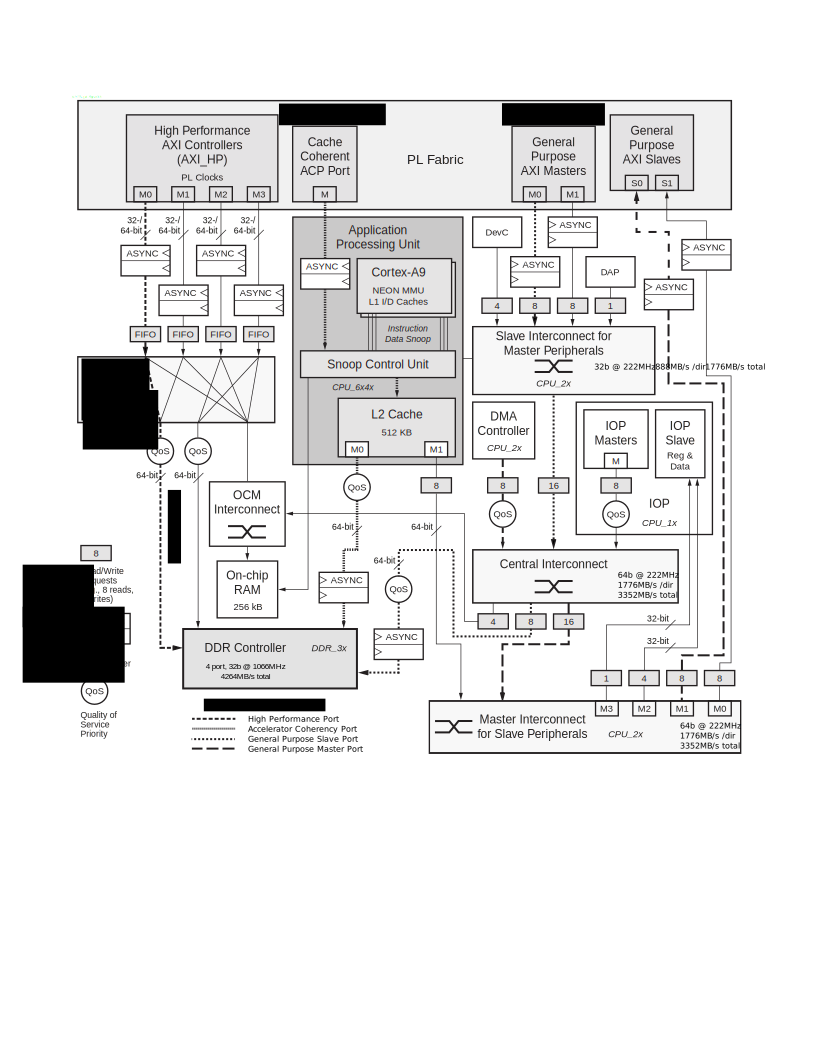
\includegraphics[scale=.9,center,trim={0 75mm 0 0},clip]{img/zynq-7000.pdf}
  \caption{The Zynq 7000 system architecture. 
  Note that port naming follows the controller role, not the port's.
  For example, the ``GP \acr{axi} Masters'' are connected to the
  ``GP \acr{axi} Slave Ports'', titled ``M0'' and ``M1''. Conversely,
  the ``GP \acr{axi} Slaves'' are connected to the ``GP \acr{axi} Master Ports'', titled ``S0'' and ``S1''.
  Modified image from \cite{ug585}.
  }
  \label{fig:zynq7000-block}
\end{figure}

\subsubsection{The High Performance Ports}

The Zynq 7000 provides four \gls{hp}s, \gls{hp}0 to \gls{hp}3.
These are all \acr{axi} slave ports to the PL,
connecting a Full \acr{axi}3 master at the PL endpoint. 
If the \acr{axi} master is implemented in \acr{axi}4, as is the usual case,
a protocol conversion must take place before connection.

The ports are clocked by a PL clock, at up to 150MHz, and can be 32 or 64 bit wide.
As the \acr{axi} protocol mandates, they have separate wires for each direction,
offering a per direction bandwidth of 1200MB/s for each port.

The \gls{hp} ports are connected to the memory controller through the Memory Interconnect
which in turn drives two of the four ports of the memory controllers, as well as
one port of the \acrfull{ocm} interconnect.
The port clock will be converted to 355MHz,
offering a switching speed of 2840MB/s per direction, 5680MB/s total.
The switching scheme routes the traffic from the first
two \gls{hp} ports to the first memory port, and the other two \gls{hp} ports
to the second. 

The memory controller offers an aggregate bandwidth of 4264MB/s 
shared among its four ports, irrespectively of the data flow direction.
Therefore, if all \gls{hp} ports are used and configured at their maximum ratings,
the maximum theoretical bandwidth of 9600MB/s will be first capped by the
memory interconnect, and if the OCM path is not used, will be further constricted
by the memory controller.

\subsubsection{The Accelerator Coherent Port}

The ACP port, compared to the \gls{hp} ports, 
has equivalent performance specifications.
The connectivity to the memory subsystem, 
however, is totally different.
As it was mentioned in \ref{amba}, 
the ACP port needs to be in close proximity to the
processor in order to provide cache coherency 
to traffic generated from a non-coherent \acr{axi} master.
Indeed, in Zynq-7000 series the \gls{acp} port is connected 
directly to the Snoop Control Unit of the L2 Cache. 
From there, it can access one dedicated 
port of the memory controller.
This is a low latency path to memory, 
but its tight relationship with the processor
will complicate the usage scenarios.

\subsubsection{The General Purpose Slave Ports}

The GP slave ports offer the half of the data width 
of the \gls{hp} ports as they are 32 bit only,
but they can operate at up to the same frequency of 150MHz. 
Nonetheless, in order to reach the memory controller 
they follow a much more complicated path.

Firstly they reach the Slave Interconnect. 
They occupy two of its four slave ports,
the other being dedicated to the 
\acrf{devc} controller and 
the \acrf{dap}.
Note that the former will be heavily used as it is responsible
for programming the FPGA during partial reconfiguration.
The Slave Interconnect operates at 222MHz, 
offering an aggregate bandwidth of 888MB/s per direction.

The master port of Slave Interconnect is connected to
Central Interconnect. The Central Interconnect operates
also at 222MHz but has a width of 64 bits, totalling at 1776MB/s
per direction. Nevertheless, the Central Interconnect,
as the name would imply, is shared among many peripherals.
Apart the Slave Interconnect, it is also a slave for the
PS DMA controller and the I/O Peripherals: 
The flash memory interfaces, the USB and Ethernet controllers, etc.
The Central Interconnect is master to three peripherals:
One memory port, the OCM interconnect, and the Master Interconnect.

\subsubsection{The General Purpose Master Ports}

The GP master ports are the funcional opposite of GP slave ports;
they can connect PL slaves and they route the traffic through the
Master Interconnect which in turn is a slave to the Central Interconnect.
It is important to note that they are the only master ports from the PS side.
If any transaction has to be started with the initiative of the PS,
it \emph{must} pass from these ports.

\subsection{The Zynq UltraScale+ Architecture}

The UltraScale+ series has significantly improved the system interconnect.
Apart from the expected increase in number and bandwidth of the
PS-PL ports and their pathway to the memory, there is much better support
for cache-coherent peripherals. An overview focused on interconnect
is displayed in figure \ref{fig:zynqmp-block}.

\begin{figure}[htbp]
  \centering
  \captionsetup{justification=centering,margin=0cm}
  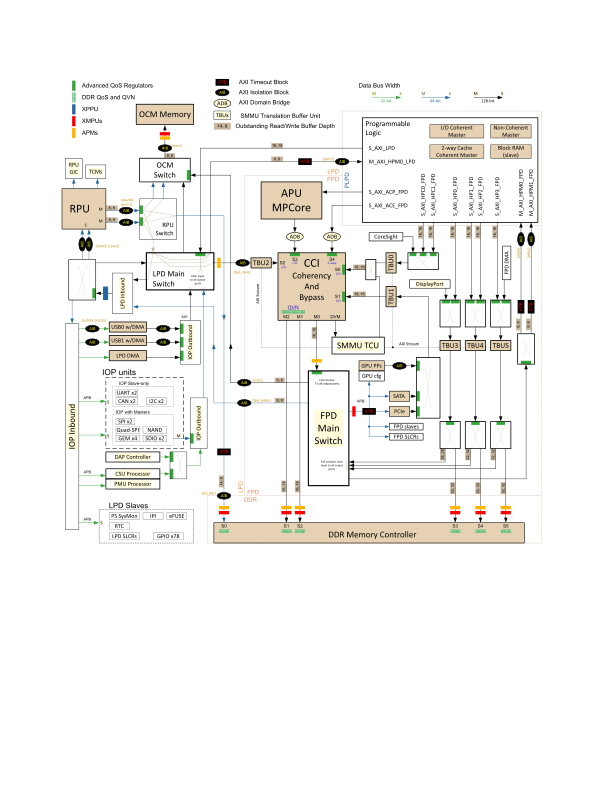
\includegraphics[scale=.9,center,trim={0 75mm 0 0},clip]{img/zynqmp.pdf}
  \caption{The Zynq UltraScale+ system architecture, image from Xilinx\cite{ug1085}.}
  \label{fig:zynqmp-block}
\end{figure}


\subsection{High Performance FPD Ports}
The UltraScale+ also features the 7000's \gls{hp} ports. 
The ports are upgraded to the version 4 of \acr{axi} standard, allowing a maximum burst length
of 256, up from 16 of \acr{axi}3. The width is increased to 128 bits, whereas the maximum
frequency \acr{axi} lala

\label{sect:interconnect}

